\section[Theorie]{Theorie \textnormal{\cite{germanium}}}
\label{sec:theorie}

Zum Verständnis des hochreinen Germaniumdektektors werden die theorethschen Grundlagen dessen im Folgenden erläutert.

\subsection{Die Wechselwirkung von Strahlung mit Materie}
\label{sec:WW mit Materie}

Bei der Gamma-Strahlungs-Detektion werden Elektronen des Detektor-Matrials von den Gamma-Photonen angeregt und damit werden die 
Atome ionisiert. Daher bilden sich Elektronen-Loch-Paare. Die Primärenelektronen ionisieren wiederum weitere Atome des Detektor-Mediums und erzeugen somit weitere Elektron Loch Paare.
Die Anzahl der Elektronen-Loch Paare ist direkt proportional zur Energie des Elektrons aus der primären
Wechselwirkung.

Da der Absorbtionskoeffizient für Gamma-Strahlung bei Gasen sehr niedrig ist, 
werden Gamma-Strahlen-Detektoren aus Festkörpern gebaut. Das Matrial des Detektors muss so gewählt werden, dass
die Anzahl Elektronen-Loch-Paare gesammelt und als elektrisches Signal wiedergegeben werden kann.
Zusätzlich ist der Grad der Interaktion von Gamma-Strahlung mit Materie abhängig von der Energie der Strahlung.
Der Intensitätsverlust  eine $\gamma$-Strahls in Materie ist abhängig von der jeweiligen Schichtdicke des Materials $d$,
der Elektronendichte und dem Wirkungsquerschnitt $\sigma$. Dabei ist der Wirkungsquerschnitt ein Maß für die Wahrscheinlichkeit einer Teilchenreaktion.
Dieser lässt sich als effektive Wirkungsfläche interpretieren

In Abbildung \ref{fig:koeffizient} ist der Dämpfungskoeffizient von Germanium, welcher die Reduktion der Strahlungsintensität
bei bestimmter Energie verursacht durch den Absorber misst, gegen die Gamma-Strahlen Energie aufgetragen.


\begin{figure}[H]
    \centering
    \includegraphics[width=0.5\textwidth]{content/grafik/dämpfungskoeffizientGermanium.jpg}
    \caption{ \cite{gamma_ray}}
    \label{fig:koeffizient}
\end{figure}

Die totale Kurve setzt sich aus verschiedenen Komponenten zusammen: Der Photoeffekt, der Compton Effekt und die Paarerzeugung.
Im Folgenden werden die einzelnen Komponenten erläutert.

\subsubsection{Der Photoeffekt}
\label{sec:photoeffekt}

Der Photoeffekt beschreibt den Prozess bei dem ein ein Gamma-Quant mit einem Hüllenelektron wechselwirkt.
Das Photon wird absorbiert, daher gibt es seine gesamte Energie an das Atom ab, und ein Elektron wird emittiert. 
Das Atom nimmt dabei den Rückstoßimpuls auf und wird ionisiert.
Anhand der Abbildung \ref{fig:koeffizient} lässt sich ablesen, dass für Energie im Bereich bis zu \qty{100}{\kilo\eV} 
Absorbtion durch den Photoeffekt dominiert. Der Wirkungsquerschnitt des Photoeffekts fällt für große Energien ab.
Bei konstanter Photonen-Energie nimmt $\sigma$ stark zu für wachsende $Z$.
Demnach ist der Wirkungsquerschnitt abhängig von Energie der der $\gamma$-Quanten und der Kernladungszahl $Z$.
%Für natürliche Strahler ergibt sich $ \sigma_{\text{Ph}} \sim Z^{\alpha} / E^{\delta} $

\subsubsection{Der Compton Effekt}
\label{sec:compton}

Der Compton-Effekt ist die Streuunug eines Photons an einem quasi-freien oder freien Elektron.
Die Hüllenelektronen eines Atoms werden hier als quasi-frei betrachtet unter der Bedingung, dass
die Enrgie des Photons viel größer als die Bindungsenergie der Elektronen ist. Dieser Prozess
dominiert in Materie um \qty{1}{\mega\eV}.
Die Kinematik der Compton Streuung ist in Abilldung \ref{fig:compton} zu sehen.

\begin{figure}[H]
    \centering
    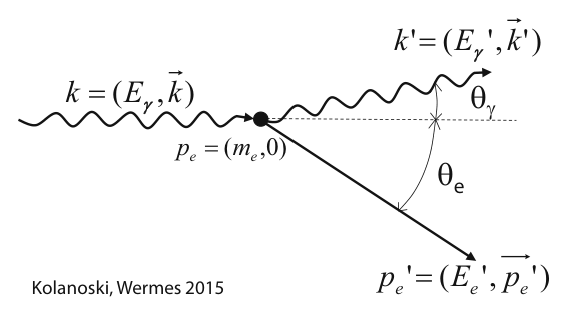
\includegraphics[width=0.5\textwidth]{content/grafik/compton.jpg}
    \caption{Die Kinematik des Compton Effekts, wobei das Elektron als quasi-frei betrachtet wird.\cite{teilchendetektoren}}
    \label{fig:compton}
\end{figure}

Um den Zusammenhang zwischen der Energie und des Winkels des gestreuten Photons
zu brechenen, werden Viererimpulse verwendet. Diese wurden in der Abbildung \ref{fig:compton} definiert.
Dabei bezeichnen $k$ und $p_{\text{e}}$ die Viererimpule des Photons und des Elektrons vor dem Stoß.
$k'$ und $p_{\text{e}}'$ bezeichen die Viererimpulse nach dem Stoß.
Aus Impulerhaltung und Energieerhaltung folgt der Zusammenhang
\begin{equation}
    E_\gamma^{\prime}=\frac{E_\gamma}{1+\epsilon\left(1-\cos \theta_\gamma\right)}
    \label{eqn:Energie_comptonstreuung}
\end{equation}
für die Energie des gestreuten Photons.

Den Wirkungsquerschnitt der Compton Streuung ergibt sich aus der Integration der Klein-Nishina-Formel über den Raumwinkel
\begin{equation}
    \frac{d \sigma}{d \Omega}=\frac{r_e^2}{2\left[1+\epsilon\left(1-\cos \theta_\gamma\right)\right]^2}\left(1+\cos ^2 \theta_\gamma+\frac{\epsilon^2\left(1-\cos \theta_\gamma\right)^2}{1+\epsilon\left(1-\cos \theta_\gamma\right)}\right).
\end{equation}
Der totale Compton-Wirkungsquerschnitt pro Elektron lauetet
\begin{equation}
    \sigma_{\text{Compton}}=2 \pi r_e^2\left[\frac{1+\epsilon}{\epsilon^2}\left(\frac{2(1+\epsilon)}{1+2 \epsilon}-\frac{1}{\epsilon} \ln (1+2 \epsilon)\right)+\frac{1}{2 \epsilon} \ln (1+2 \epsilon)-\frac{1+3 \epsilon}{(1+2 \epsilon)^2}\right].
    \label{eqn:Compton_Wirkungsquerschnitt}
\end{equation}

Für den Wirkungsquerschnit pro Atom kommt es zu einer linearen Abhängigkeit
\begin{equation}
    \sigma_{\text{Compton}}^{\text{Atom}}=Z \sigma_{\text{Compton}}.
\end{equation}

Die Linearität gilt für die Annahme von freien Elektronen, also für Energien oberhalb der
Bindungsenergie des Elektronen.
Für kleinere Energien der Compton Wirkungsquerschnitt in Materie ab.

\subsubsection{Die Paarerzeugung}
\label{paarerzeugung}